\begin{frame}{Contextualização}
    \begin{itemize} \setlength\itemsep{1em}
        \item Criar conteúdo para jogos manualmente exige muito esforço de trabalho
        \item Quanto maior o mundo virtual, tecnicamente mais tempo os jogadores irão explorar \cite{fernando2009costas}
    \end{itemize}
    
    \begin{figure}[H]
        \centering
        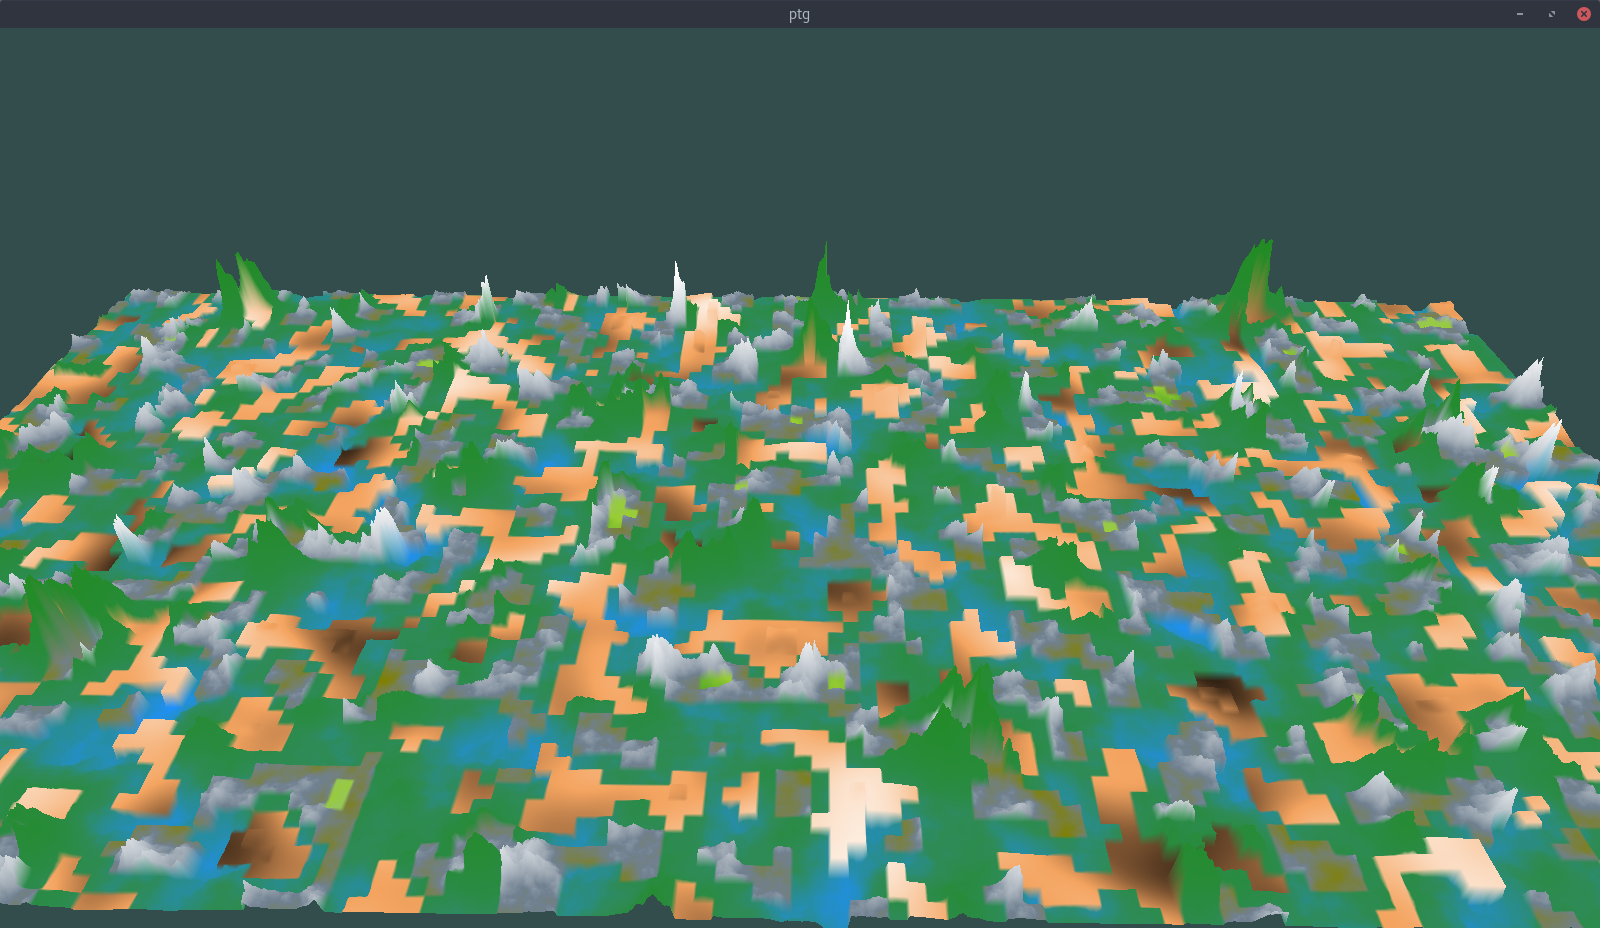
\includegraphics[width=.5\textwidth]{img/re2bfb/fb/4b32.png}
        \caption{Terreno vasto.}
        \label{fig:img_re2bfb_fb_4b32Again}
    \end{figure}
    
\end{frame}

\begin{frame}{Introdução}
    \begin{itemize} \setlength\itemsep{1em}
        \item Esse trabalho apresenta uma técnica de criação de terrenos para jogos
        \item Cria diferentes padrões de relevos para representar biomas
        \item Distribui os biomas em áreas
        \item Implementa uma fronteira suave entre biomas
    \end{itemize}
    
\end{frame}